% !TeX program = xelatex
% !TeX encoding = UTF-8
\documentclass{article}
\usepackage{ctex}
\usepackage{geometry}
\geometry{a4paper, left=3cm, right=3cm, top=2.5cm, bottom=2.5cm}

\usepackage{graphicx}
\usepackage{enumerate}
\usepackage{amsmath, amssymb, amsthm}
\usepackage{algorithm, algorithmic}
\floatname{algorithm}{算法}
\renewcommand{\algorithmicrequire}{\textbf{Input:}}
\renewcommand{\algorithmicensure}{\textbf{Output:}}

\usepackage{listings}
\usepackage{xcolor}
\usepackage{hyperref}
\hypersetup{colorlinks, citecolor=black, filecolor=black, linkcolor=black, urlcolor=black}

% 代码样式
\lstset{
    language=Python,
    keywordstyle=\color{blue},
    commentstyle=\color{green!50!black},
    stringstyle=\color{red},
    numbers=left,
    numberstyle=\tiny,
    basicstyle=\ttfamily\small,
    frame=single,
    breaklines=true,
    extendedchars=false
}

\title{第四次上机作业}
\author{学号：241830137\quad 姓名：朱子健}
\date{\today}

\begin{document}

\maketitle

\section{问题}
考虑函数\(R(x)=\frac{1}{1+x^2}\).利用下列条件做插值逼近，并且与\(R(x)\)的图像比较.
\begin{enumerate}[(1)]
    \item 用等距节点\(x_i = -5 + i, i = 0, 1,...,10\).\\
          画出三次自然样条插值函数的图像；
    \item 用等距节点\(x_i = -5 + i, i = 0, 1,...,10\).\\
          画出分段三次Hermite插值（相邻两点的函数值与一阶导数值）函数的图像；
\end{enumerate}
\section{算法原理与设计}
\subsection{三次自然样条插值函数}
\subsubsection{算法原理}
在每个子区间 $[x_i, x_{i+1}]$ 上，三次样条 $S_i(x)$ 可表示为：
\begin{equation}
S_i(x) = \sum_{l=1}^{4} C_{i,l}(x - x_i)^{l-1}
\end{equation}
令 $\alpha_i = S''(x_i)$，根据讲义，系数由下式确定：
\begin{itemize}
    \item $C_{i,1} = f_i$
    \item $C_{i,2} = \frac{f_{i+1} - f_i}{h_i} - \frac{h_i}{6}(\alpha_{i+1} + 2\alpha_i)$
    \item $C_{i,3} = \frac{\alpha_i}{2}$
    \item $C_{i,4} = \frac{\alpha_{i+1} - \alpha_i}{6h_i}$
\end{itemize}
其中 $\alpha_i$ 由三对角方程组 $h_{i-1}\alpha_{i-1} + 2(h_{i-1}+h_i)\alpha_i + h_i\alpha_{i+1} = 6(f[x_i, x_{i+1}] - f[x_{i-1}, x_i])$ 确定。

\subsubsection{算法设计}
\begin{algorithm}[H]
\caption{计算自然样条插值函数}
\begin{algorithmic}[1]
    \STATE \textbf{输入} 节点数组 $X = [x_1, \dots, x_{n+1}]$，函数值 $Y = [f_1, \dots, f_{n+1}]$
    \STATE \textbf{输出} 每段三次多项式系数 $C_{i,1}, C_{i,2}, C_{i,3}, C_{i,4}$ ($i=1, \dots, n$)
    \STATE 设置边界条件：$\alpha_1 = 0, \alpha_{n+1} = 0$
    \STATE 求解三对角方程组得到 $\alpha_2, \dots, \alpha_n$
    \FOR{$i = 1$ to $n$}
        \STATE $h_i \leftarrow x_{i+1} - x_i$
        \STATE $C_{i,1} \leftarrow f_i$
        \STATE $C_{i,2} \leftarrow \frac{f_{i+1} - f_i}{h_i} - \frac{h_i}{6}(\alpha_{i+1} + 2\alpha_i)$
        \STATE $C_{i,3} \leftarrow \alpha_i / 2$
        \STATE $C_{i,4} \leftarrow (\alpha_{i+1} - \alpha_i) / (6h_i)$
    \ENDFOR
\end{algorithmic}
\end{algorithm}

\subsection{分段三次 Hermite 插值}
\subsubsection{算法原理}
在每一区间 $[x_i, x_{i+1}]$ 上，构造三次多项式满足 $H(x_i)=f_i, H(x_{i+1})=f_{i+1}, H'(x_i)=f'_i, H'(x_{i+1})=f'_{i+1}$。对于 $R(x)$，其一阶导数为 $R'(x) = \frac{-2x}{(1+x^2)^2}$。系数计算如下：
\begin{align*}
    A_i &= f_i, \quad B_i = f'_i \\
    C_i &= \frac{3(f_{i+1}-f_i)/h_i - 2f'_i - f'_{i+1}}{h_i} \\
    D_i &= \frac{f'_{i+1} + f'_i - 2(f_{i+1}-f_i)/h_i}{h_i^2}
\end{align*}

\subsubsection{算法设计}
\begin{algorithm}[H]
\caption{计算三次Hermite插值多项式}
\begin{algorithmic}[1]
    \STATE \textbf{输入}: 节点 $x_1, \dots, x_{n+1}$，函数值 $f_1, \dots, f_{n+1}$
    \STATE \textbf{输出}: 系数 $C_{i,1}, C_{i,2}, C_{i,3}, C_{i,4}$ ($i=1, \dots, n$)
    \STATE 设置边界条件：$\alpha_1 = 0, \alpha_{n+1} = 0$
    \STATE 求解三对角方程组得到 $\alpha_2, \dots, \alpha_n$
    \FOR{$i = 1$ to $n$}
        \STATE $h_i \leftarrow x_{i+1} - x_i$
        \STATE $C_{i,1} \leftarrow f_i$
        \STATE $C_{i,2} \leftarrow \frac{f_{i+1} - f_i}{h_i} - \frac{h_i}{6}(\alpha_{i+1} + 2\alpha_i)$
        \STATE $C_{i,3} \leftarrow \alpha_i / 2$
        \STATE $C_{i,4} \leftarrow (\alpha_{i+1} - \alpha_i) / (6h_i)$
    \ENDFOR
\end{algorithmic}
\end{algorithm}

\section{结果分析}
根据题目给定的节点和原函数 $R(x)=\frac{1}{1+x^2}$，我们可以写出这两种插值函数的具体数学表达式。
\subsection{三次自然样条插值具体表达式}
与 Hermite 插值类似，三次自然样条插值函数 $S(x)$ 在第 $i$ 个子区间 $[x_i, x_{i+1}]$ 上的表达式 $S_i(x)$ 为：

\begin{equation}
    S(x) = S_i(x) = C_{i,1} + C_{i,2}(x - x_i) + C_{i,3}(x - x_i)^2 + C_{i,4}(x - x_i)^3, \quad x \in [x_i, x_{i+1}]
\end{equation}

记 $M_i = S''(x_i)$ 为节点处的二阶导数。各项系数 $C_{i,k}$ 由下式给出（$h=1$）：
\begin{align}
    C_{i,1} &= y_i = \frac{1}{1+x_i^2} \\
    C_{i,2} &= (y_{i+1} - y_i) - \frac{1}{6}(M_{i+1} + 2M_i) \\
    C_{i,3} &= \frac{M_i}{2} \\
    C_{i,4} &= \frac{M_{i+1} - M_i}{6}
\end{align}

其中，二阶导数 $M_i$ 序列并不是直接已知的，而是通过求解由连续性条件推导出的三对角线性方程组（即三弯矩方程）获得。对于等距节点 $h=1$，内部节点 $i = 1, 2, \dots, 9$ 满足：
\begin{equation}
    M_{i-1} + 4M_i + M_{i+1} = 6(y_{i-1} - 2y_i + y_{i+1})
\end{equation}
由于本题要求的是\textbf{自然样条}（Natural Spline），因此附加边界条件为端点处的二阶导数为零：
\begin{equation}
    M_0 = 0, \quad M_{10} = 0
\end{equation}
联立 (11) 和 (12) 式求解出一个维度为 $9 \times 9$ 的对称正定三对角方程组，解出唯一的 $M_1, \dots, M_9$ 后代入 (8)-(10) 式，即完成了所有区间样条多项式解析表达式的确定。

\subsection{分段三次 Hermite 插值具体表达式}
分段三次 Hermite 插值函数 $H(x)$ 在整个区间 $[-5, 5]$ 上是分段定义的。对于任意 $x \in [-5, 5]$，若 $x$ 落在第 $i$ 个子区间 $[x_i, x_{i+1}]$ 内（$i = 0, 1, \dots, 9$），其具体表达式为一个三次多项式 $H_i(x)$：

\begin{equation}
    H(x) = H_i(x) = A_i + B_i(x - x_i) + C_i(x - x_i)^2 + D_i(x - x_i)^3, \quad x \in [x_i, x_{i+1}]
\end{equation}

由于步长 $h=1$，根据 Hermite 插值基函数推导，上述各项系数可由节点处的值直接计算：
\begin{align}
    A_i &= y_i = \frac{1}{1+x_i^2} \\
    B_i &= y'_i = \frac{-2x_i}{(1+x_i^2)^2} \\
    C_i &= 3(y_{i+1} - y_i) - 2y'_i - y'_{i+1} \\
    D_i &= y'_i + y'_{i+1} - 2(y_{i+1} - y_i)
\end{align}
将给定的 $y_i$ 和 $y'_i$ 数值代入 (2)-(5) 式，即可完全确定各区间的 Hermite 多项式。

\subsection{图像对比}
通过编写 C++ 程序计算并绘制插值曲线，我们可以得出如下分析结论：
\begin{figure}[h]
    \centering
    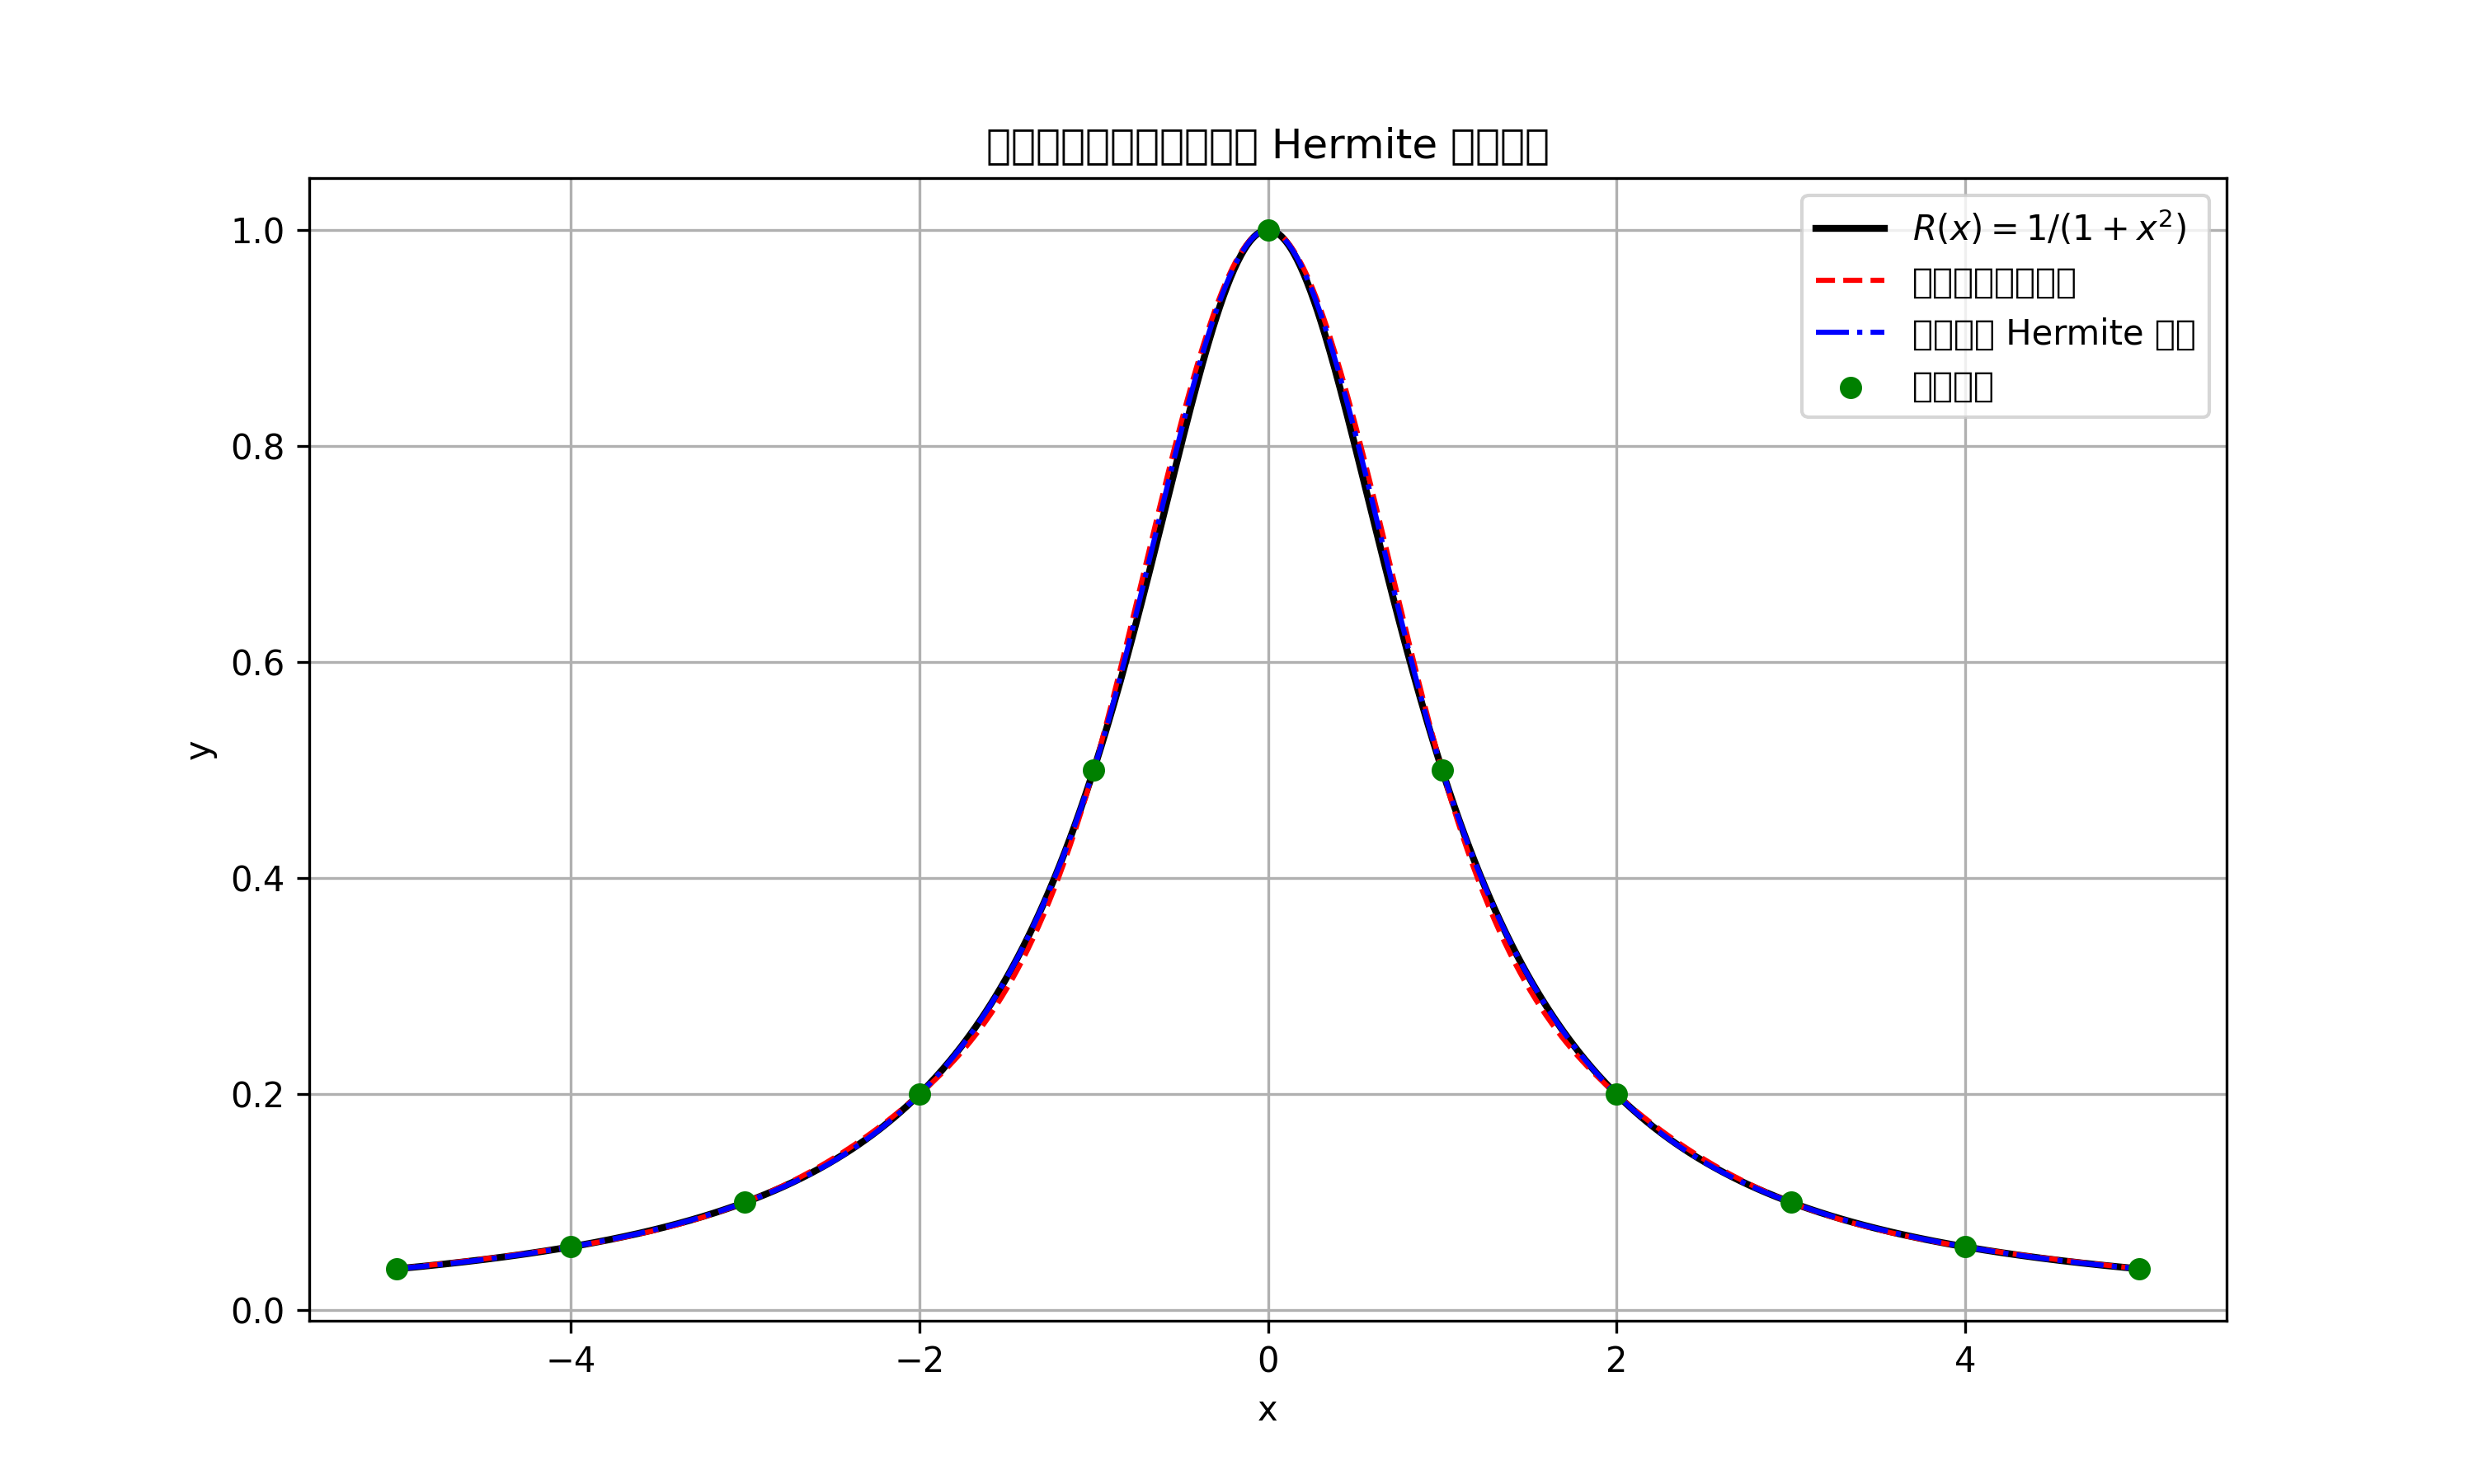
\includegraphics[width=0.8\textwidth]{comparison.png}
    \caption{三次自然样条与分段三次 Hermite 插值逼近结果}
\end{figure}

\begin{enumerate}
    \item \textbf{整体逼近能力}：由于 $R(x)$ 在 $[-5, 5]$ 区间内是光滑函数，三次自然样条插值 (Natural Cubic Spline) 在全区间上表现出极高的逼近精度。在靠近中心点 $x=0$ 的剧烈变化区域，样条插值曲线紧密跟随原函数曲线。
    \item \textbf{边界行为}：三次自然样条在边界处满足 $S''(x_0) = S''(x_{10}) = 0$，这使得其在边界处的曲率趋于零。图像显示这种边界处理方式在 $R(x)$ 这种远离中心快速衰减的函数上效果良好。
    \item \textbf{Hermite 插值的平滑度}：分段三次 Hermite 插值在每一节点处通过导数值 $f'(x_i)$ 强制保证了 $C^1$ 连续性。从图中可以看出，其逼近曲线非常平滑，且在节点处的导数过渡与原函数一致，说明引入导数信息显著提高了插值在局部区间内的预测能力。
    \item \textbf{误差分布}：误差较大的区域主要集中在函数曲率最大的区间 $[-1, 1]$ 附近。相比于全局高次 Lagrange 插值（会出现显著的 Runge 震荡），这两种分段低次插值方法均成功消除了端点附近的震荡，证明了它们在数值计算中的稳定性。
\end{enumerate}

\newpage
\section{附录：Python 源代码实现}
\begin{lstlisting}[language=Python]
import numpy as np
import matplotlib.pyplot as plt

# 原函数及其导数
def R(x):
    return 1.0 / (1.0 + x * x)

def dR(x):
    return -2.0 * x / (1.0 + x * x) ** 2

# 追赶法求解三对角方程组 Ax = d
def solve_tridiagonal(a, b, c, d):
    n = len(d)
    cp = np.zeros(n)
    dp = np.zeros(n)
    x = np.zeros(n)
    cp[0] = c[0] / b[0]
    dp[0] = d[0] / b[0]
    for i in range(1, n):
        m = b[i] - a[i] * cp[i-1]
        if i < n-1:
            cp[i] = c[i] / m
        dp[i] = (d[i] - a[i] * dp[i-1]) / m
    x[-1] = dp[-1]
    for i in range(n-2, -1, -1):
        x[i] = dp[i] - cp[i] * x[i+1]
    return x

# 三次自然样条插值类
class NaturalSpline:
    def __init__(self, x_nodes, y_nodes):
        self.x = np.array(x_nodes)
        self.y = np.array(y_nodes)
        self.n = len(x_nodes) - 1
        self.h = x_nodes[1] - x_nodes[0]   # 等距节点，步长固定

        # 构造三对角方程组 (内部节点数 = n-1)
        m = self.n - 1
        a = np.ones(m)          # 下对角线
        b = 4.0 * np.ones(m)    # 主对角线
        c = np.ones(m)          # 上对角线
        d = np.zeros(m)
        for i in range(1, self.n):
            d[i-1] = 6.0 / (self.h * self.h) * (self.y[i-1] - 2*self.y[i] + self.y[i+1])

        # 求解内部节点的二阶导数 M1...M_{n-1}
        m_inner = solve_tridiagonal(a, b, c, d)
        # 边界条件 M0 = Mn = 0 (自然样条)
        self.M = np.concatenate(([0.0], m_inner, [0.0]))

    def eval(self, x):
        # 确定 x 所在的区间下标
        if x == self.x[-1]:
            i = self.n - 1
        else:
            i = int(np.floor((x - self.x[0]) / self.h))
        i = max(0, min(i, self.n - 1))

        xi = self.x[i]
        xi1 = self.x[i+1]
        hi = self.h
        Mi = self.M[i]
        Mi1 = self.M[i+1]
        yi = self.y[i]
        yi1 = self.y[i+1]

        t1 = xi1 - x
        t2 = x - xi
        term1 = (Mi * t1**3 + Mi1 * t2**3) / (6 * hi)
        term2 = (yi / hi - Mi * hi / 6) * t1
        term3 = (yi1 / hi - Mi1 * hi / 6) * t2
        return term1 + term2 + term3

# 分段三次 Hermite 插值 (使用基函数形式)
def hermite_eval(x, xn, yn, ypn):
    h = xn[1] - xn[0]   # 等距步长
    if x == xn[-1]:
        i = len(xn) - 2
    else:
        i = int(np.floor((x - xn[0]) / h))
    i = max(0, min(i, len(xn)-2))

    t = (x - xn[i]) / h
    # Hermite 基函数插值
    return (yn[i] * (1 + 2*t) * (1-t)**2 +
            yn[i+1] * (3 - 2*t) * t**2 +
            ypn[i] * h * t * (1-t)**2 +
            ypn[i+1] * h * (t-1) * t**2)

# 主程序
def main():
    # 等距节点 x_i = -5 + i, i = 0..10
    xi = np.array([-5.0 + i for i in range(11)])
    yi = R(xi)
    ypi = dR(xi)

    # 创建自然样条对象
    spline = NaturalSpline(xi, yi)

    # 生成绘图所需的密集点
    x_plot = np.linspace(-5, 5, 1000)
    y_original = R(x_plot)
    y_spline = np.array([spline.eval(x) for x in x_plot])
    y_hermite = np.array([hermite_eval(x, xi, yi, ypi) for x in x_plot])

    # 绘图
    plt.figure(figsize=(10, 6))
    plt.plot(x_plot, y_original, 'k-', linewidth=2, label='$R(x)=1/(1+x^2)$')
    plt.plot(x_plot, y_spline, 'r--', linewidth=1.5, label='三次自然样条插值')
    plt.plot(x_plot, y_hermite, 'b-.', linewidth=1.5, label='分段三次 Hermite 插值')
    plt.scatter(xi, yi, c='green', s=30, zorder=5, label='插值节点')
    plt.xlabel('x')
    plt.ylabel('y')
    plt.title('三次自然样条与分段三次 Hermite 插值对比')
    plt.legend()
    plt.grid(True)
    plt.savefig('comparison.png', dpi=300)
    plt.show()

    # 可选：输出部分数值结果（与原 C++ 代码类似）
    print("x\tOriginal\tSpline\t\tHermite")
    for x in np.arange(-5, 5.1, 0.5):
        print(f"{x:.6f}\t{R(x):.6f}\t{spline.eval(x):.6f}\t{hermite_eval(x, xi, yi, ypi):.6f}")

if __name__ == "__main__":
    main()
\end{lstlisting}
\end{document}